% Options for packages loaded elsewhere
\PassOptionsToPackage{unicode}{hyperref}
\PassOptionsToPackage{hyphens}{url}
\PassOptionsToPackage{dvipsnames,svgnames*,x11names*}{xcolor}
%
\documentclass[
]{article}
\usepackage{amsmath,amssymb}
\usepackage{lmodern}
\usepackage{ifxetex,ifluatex}
\ifnum 0\ifxetex 1\fi\ifluatex 1\fi=0 % if pdftex
  \usepackage[T1]{fontenc}
  \usepackage[utf8]{inputenc}
  \usepackage{textcomp} % provide euro and other symbols
\else % if luatex or xetex
  \usepackage{unicode-math}
  \defaultfontfeatures{Scale=MatchLowercase}
  \defaultfontfeatures[\rmfamily]{Ligatures=TeX,Scale=1}
\fi
% Use upquote if available, for straight quotes in verbatim environments
\IfFileExists{upquote.sty}{\usepackage{upquote}}{}
\IfFileExists{microtype.sty}{% use microtype if available
  \usepackage[]{microtype}
  \UseMicrotypeSet[protrusion]{basicmath} % disable protrusion for tt fonts
}{}
\makeatletter
\@ifundefined{KOMAClassName}{% if non-KOMA class
  \IfFileExists{parskip.sty}{%
    \usepackage{parskip}
  }{% else
    \setlength{\parindent}{0pt}
    \setlength{\parskip}{6pt plus 2pt minus 1pt}}
}{% if KOMA class
  \KOMAoptions{parskip=half}}
\makeatother
\usepackage{xcolor}
\IfFileExists{xurl.sty}{\usepackage{xurl}}{} % add URL line breaks if available
\IfFileExists{bookmark.sty}{\usepackage{bookmark}}{\usepackage{hyperref}}
\hypersetup{
  pdftitle={Crab body metrics - predicting the subspecies of crabs},
  pdfauthor={IJsbrand Pool, 403589},
  colorlinks=true,
  linkcolor=blue,
  filecolor=Maroon,
  citecolor=Blue,
  urlcolor=Blue,
  pdfcreator={LaTeX via pandoc}}
\urlstyle{same} % disable monospaced font for URLs
\usepackage[margin=1in]{geometry}
\usepackage{graphicx}
\makeatletter
\def\maxwidth{\ifdim\Gin@nat@width>\linewidth\linewidth\else\Gin@nat@width\fi}
\def\maxheight{\ifdim\Gin@nat@height>\textheight\textheight\else\Gin@nat@height\fi}
\makeatother
% Scale images if necessary, so that they will not overflow the page
% margins by default, and it is still possible to overwrite the defaults
% using explicit options in \includegraphics[width, height, ...]{}
\setkeys{Gin}{width=\maxwidth,height=\maxheight,keepaspectratio}
% Set default figure placement to htbp
\makeatletter
\def\fps@figure{htbp}
\makeatother
\setlength{\emergencystretch}{3em} % prevent overfull lines
\providecommand{\tightlist}{%
  \setlength{\itemsep}{0pt}\setlength{\parskip}{0pt}}
\setcounter{secnumdepth}{5}
\usepackage{graphicx}
\usepackage{float}
\usepackage{booktabs}
\usepackage{longtable}
\usepackage{array}
\usepackage{multirow}
\usepackage{wrapfig}
\usepackage{float}
\usepackage{colortbl}
\usepackage{pdflscape}
\usepackage{tabu}
\usepackage{threeparttable}
\usepackage{threeparttablex}
\usepackage[normalem]{ulem}
\usepackage{makecell}
\usepackage{xcolor}
\ifluatex
  \usepackage{selnolig}  % disable illegal ligatures
\fi

\title{Crab body metrics - predicting the subspecies of crabs}
\author{IJsbrand Pool, 403589}
\date{}

\begin{document}
\maketitle

{
\hypersetup{linkcolor=}
\setcounter{tocdepth}{2}
\tableofcontents
}
\newpage

\hypertarget{recapitulation}{%
\section{Recapitulation}\label{recapitulation}}

The goal of this project was to find out if the species of a
\emph{Leptograpsus variegatus} was predictable. The research question
that required answering for this project was: ``Can the species of a
\emph{L.variegatus} be determined based on some morphological
measurements of its carapace''.

The data that was delivered with this project contained five
morphological measurements, these were measured in millimeters. To be
capable of answering this question, the data was first explored and
cleaned and visualized to be able to draw conclusions from the data.
Then, multiple machine learning algorithms were tested along with some
meta-learning algorithms to see if there would be an optimal algorithm
for the answering of the research question.

The SimpleLogistic algorithm reached a accuracy of 100\% This is due to
the build-up of the data set, since its an evenly distributed data set.
This was the best accuracy gained, but since biologists and zoologists
will be using the program a tree would be preferred but since that would
mean a decrees in accuracy of 12\% a SimpleLogistic algorithm was chosen
with a strong ReadMe.

\newpage

\hypertarget{introduction}{%
\section{Introduction}\label{introduction}}

The rock crab \emph{L. variegatus}, has been recorded to occur on a
number of southern Pacific islands, along the western coast of South
America, and the coasts of Australia south of the Tropic of Capricorn.
Mahon.

By using ecological studies which extended those of Shield, and a
genetical analysis based on an electrophoretic study, established the
specific distinctness of rock crabs of the blue and orange forms of the
genus \emph{Leptograpsus}. These colour forms were previously regarded
as morphs of \emph{L. variegatus.}.

In an attempt to resolve this issue of identification and possible
misidentification of \emph{L.variegatus} a morphological study of the
Western Australian species was undertaken.

The dataset used is the crab body metrics dataset by Campbell, N.A. and
Mahon, R.J. (1974) ``A multivariate study of variation in two species of
rock crab of genus'' \emph{Leptograpsus}{[}@Crabdata{]}. This data set
contains multiple morphological metrics of the bodies of \emph{L.
variegatus.} crabs, and the gender and color of the crab. The measured
metrics are the frontal lobe size, rear width, carapace length, carapace
width and body depth. All these values are in millimeters. There are 100
orange and 100 blue crabs. 50 crabs of each gender per color of crab.

\newpage

\hypertarget{materials-and-methods}{%
\section{Materials and methods}\label{materials-and-methods}}

For this project research has been done to be able to investigate and
predict whether or not it is possible to predict the species of
\emph{L.variegatus} based on the morphological measurements of its
carapace using machine learning. Multiple machine learning algorithms
and meta-learners have been tested and checked for their accuracy. The
data was also used to be able to visualize every aspect of the
\emph{L.variegatus} its morphological measurements, to be able to answer
the research question

\hypertarget{materials}{%
\subsection{Materials}\label{materials}}

The data used in this project was publicized by Campbell, N.A. and
Mahon, R.J. (1974) A multivariate study of variation in two species of
rock crab of genus \emph{Leptograpsus}{[}@Crabdata{]}. This paper
contained useful information for this project. The data set used was a
csv file containing multiple morphological measurements for 200 crabs.
Not all attributes are as important, so it was part of the research
question to determine what attributes could be best used. Multiple
packages were used for this project, see table 1.

For the research of this project, the original publication by Campbell,
N.A. and Mahon, R.J. (1974) ``A multivariate study of variation in two
species of rock crab of genus'' was used. Along side the original data
the website for crabs was used to investigate why crabs are important
for the environment.{[}@CrabImportance{]}

Based upon the literary information the research question was formed,
this after rechecking the data set and finding out what would be an
interesting and possibly important research question.

For the data and the visualizations certain libraries have been used,
see table one for these libraries

\begin{table}[!h]

\caption{\label{tab:packages}The used packages and their versions.}
\centering
\begin{tabular}[t]{l|l}
\hline
packagelist & versionlist\\
\hline
kableExtra & 1.3.4\\
\hline
ggplot2 & 3.3.5\\
\hline
factoextra & 1.0.7\\
\hline
RWeka & 0.4-43\\
\hline
reshape & 0.8.8\\
\hline
FactoMineR & 2.4\\
\hline
gridExtra & 2.3\\
\hline
\end{tabular}
\end{table}

The packages were used to be able to manipulate and visualize the data
as well as load in data that was gathered from the WEKA program.
Furthermore, one column of the data set was deleted, the index column
since there was no apparent use for this column.

\newpage

\hypertarget{methods}{%
\subsection{Methods}\label{methods}}

Before the data could be worked with, it had to be examined and its
quality needed to be checked, there were no missing values and only one
column that did not seem useful, so only one correction had to be made
in order to understand the data better.

There are methods by which someone can determine the species of a
\emph{L.variegatus} based on some morphological measurements of its
carapace. This project tries to see if these methods can be improved
upon and if a better method can be developed

The goal is to be able to determine the the species of a
\emph{L.variegatus} based on some morphological measurements of its
carapace. So researchers and biologist have a better understanding of
the crab they are dealing with. The parameters used for this can be
found in table two

\begin{table}[!h]

\caption{\label{tab:Reading data}Codebook of the crab data set}
\centering
\fontsize{10}{12}\selectfont
\begin{tabular}[t]{l|l}
\hline
column & description\\
\hline
sp & Species\\
\hline
sex & Sex\\
\hline
index & Index\\
\hline
FL & Frontal lobe size (mm)\\
\hline
RW & Rear width (mm)\\
\hline
CL & Carapace length (mm)\\
\hline
CW & Carapace width (mm)\\
\hline
BD & Body depth (mm)\\
\hline
\end{tabular}
\end{table}

There were no further calculations needed for this project. The used
script was CrabProject.Rmd, the data files can be found within the same
area as the project file.

\newpage

\hypertarget{results}{%
\section{Results}\label{results}}

The results from this research project are placed within two different
categories, there being the exploratory data analysis and the machine
learning algorithm analysis. This choice has been made since both
sections have different outcomes and goals, but both are equally
important.

\hypertarget{exploratory-data-analysis}{%
\subsection{Exploratory data analysis}\label{exploratory-data-analysis}}

The goal of the exploratory data analusis was to be able to give an
overview of the data, which included a look at the original data and
figuring out whether or not this data is suitable for machine learning
and if not, then making it suitable for machine learning. Another goal
here was to be able to check if the research question was capable of
being answered.

Table three shows the five number summary of all the numerical
attributes within the crab data set, Since the instances within this
data set differ from each other but do seem correlated to each other the
mean and medians are somewhat close together. There are no missing
values present since they are absent from the data set.

\begin{table}[!h]

\caption{\label{tab:Five number summary of the crab data}Five number summary of the morphological measurements of the crab bodies.}
\centering
\begin{tabular}[t]{l|l|l|l|l|l}
\hline
  & Frontal Lobe & Rear Width & Carapace Length & Carapace Width & Body Depth\\
\hline
Minimum & 7.20 & 6.50 & 14.70 & 17.10 & 6.10\\
\hline
Q1 & 12.90 & 11.00 & 27.27 & 31.50 & 11.40\\
\hline
Median & 15.55 & 12.80 & 32.10 & 36.80 & 13.90\\
\hline
Mean & 15.58 & 12.74 & 32.11 & 36.41 & 14.03\\
\hline
Q3 & 18.05 & 14.30 & 37.23 & 42.00 & 16.60\\
\hline
Maximum & 23.10 & 20.20 & 47.60 & 54.60 & 21.60\\
\hline
\end{tabular}
\end{table}

\hypertarget{cleaning-the-data}{%
\subsection{Cleaning the data}\label{cleaning-the-data}}

The data in its current form, is not ready for the use of a machine
learning algorithm, this is due to the Index column, some algorithms
will over fit their model by making use of this column, so this column
needs to be deleted to be able to verify the quality of the data
gathered. The species columns was also moved to the last column so it
would be used as the class attribute.

\hypertarget{visualisations}{%
\subsection{Visualisations}\label{visualisations}}

To gain a better understanding of the correlation between the attributes
in the data set, some visualizations were made.

\begin{verbatim}
## Scale for 'colour' is already present. Adding another scale for 'colour',
## which will replace the existing scale.
\end{verbatim}

\begin{figure}[H]

{\centering 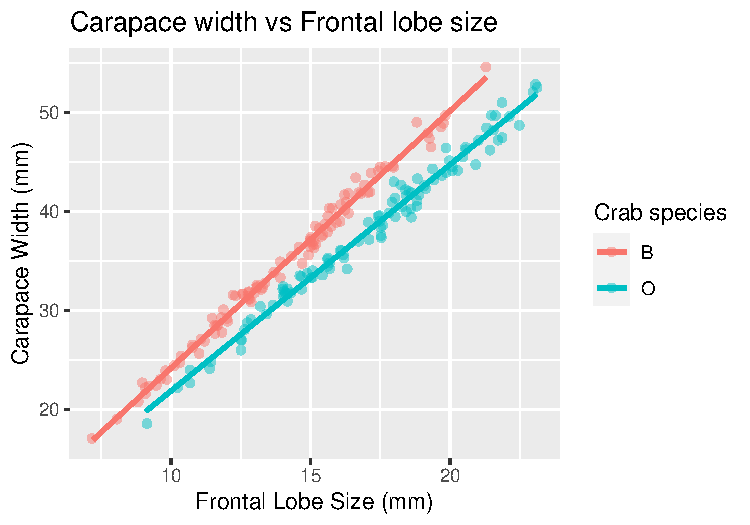
\includegraphics{CrabProject_files/figure-latex/figure1-1} 

}

\caption{Spread of Front lobe size against Carapace width based on color}\label{fig:figure1}
\end{figure}

The image above shows the spread of front lobe size against Carapace
width based on color, this visualization has been made to be able to see
if there was any correlation between these two attributes. The image
shows that the blue crabs have wider carapaces on average and shorter
frontal lobes, this could be a genetic trait for the color of this crab
and therefore this could be a good indicator to determine the subspecies
of the crab by the use of a machine learning algorithm.

Since there were only 200 crabs in this study this could of course be a
coincidence, but for the continuation of this report the assumption of
data correctness due to differences in species has been accepted.

\begin{figure}[H]

{\centering 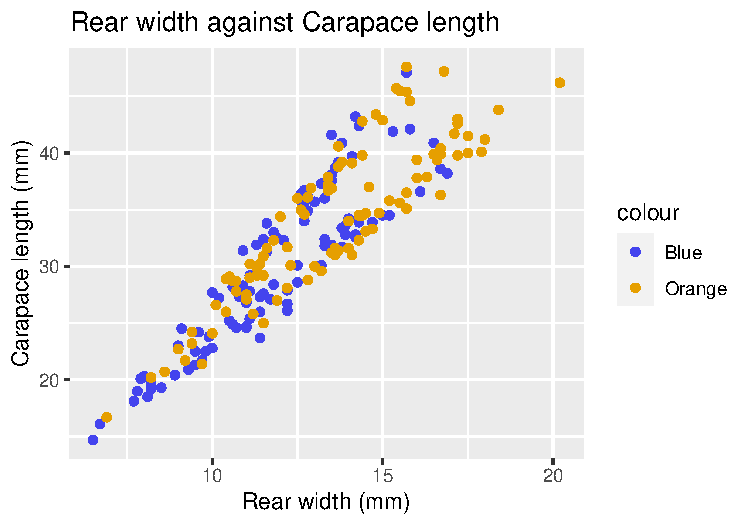
\includegraphics{CrabProject_files/figure-latex/figure2-1} 

}

\caption{Spread of Rear width against Carapace length based on color}\label{fig:figure2}
\end{figure}

Similar to the previous plot, this data also seems to show some
correlation with each other, this makes the question ``is all the data
correlated'' rise, this will have to be investigated if the data
continues to seem correlated. In the plot above the differences between
Rear width against Carapace length are visible for both the different
crabs, this being the blue group and the orange group.

\newpage
\begin{figure}[H]

{\centering 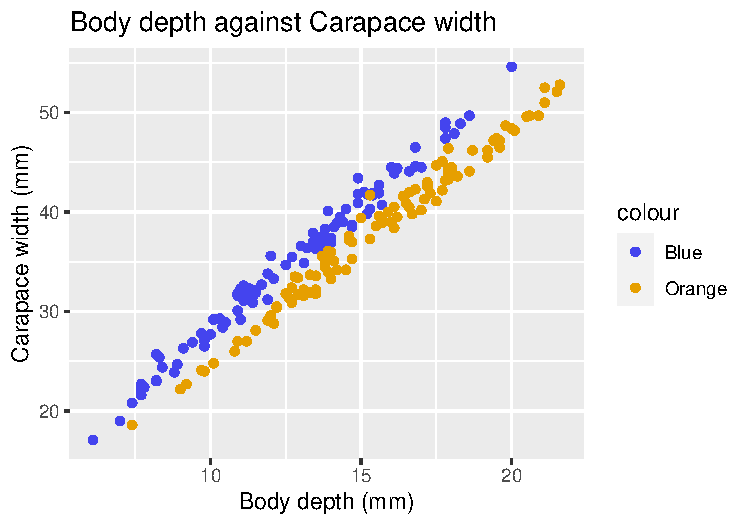
\includegraphics{CrabProject_files/figure-latex/figure3-1} 

}

\caption{Spread of Body depth against Carapace width based on color}\label{fig:figure3}
\end{figure}

This plot again shows that the blue crabs on average seem to have a
wider carapaces, but the orange crabs tend to have deeper bodies. The
attributes seem to very correlated with each other and this again
supports the theory that there may be multiple morphological attributes
that will help determine the color of the crab. However the attributes
above seem to be less clear in this then the attributes within figure
one.

As shown inside the figures one and three, the metrics of the orange and
the blue crabs appear to be in two different groups. This could indicate
that the two species could be identifiable by different elements,
including their carapace width. However, figure two indicates that the
two groups of crabs appear to have some sort of difference even within
their own respective group, this could indicate that gender plays a role
in the sizes of the morphological measurements.

\newpage
\begin{figure}[H]

{\centering 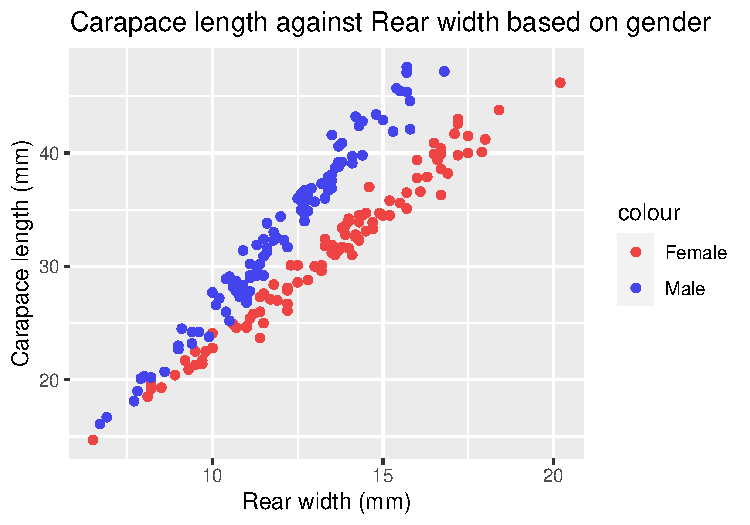
\includegraphics{CrabProject_files/figure-latex/figure4-1} 

}

\caption{Checking if the gender makes a difference}\label{fig:figure4}
\end{figure}

As seen in the density distribution of figure four, there indeed seems
to be a difference within the groups if they are divided by the male and
females of the group.

In figure 4.1 the frontal lobe size in millimeters is plotted against
the gender of the crabs, here it is clearly visible that there doesn't
seem to be much difference in the frontal lobe size between the genders,
the only difference that can be seen here appears to be in the the
smaller measurements of the frontal lobe size, slightly indicating that
the females might have a smaller frontal lobe size in general then
males, this however cannot be confirmed from this density plot.

In figure 4.2 the Rear width in millimeters is plotted against the
gender of the crabs, here it can be seen that the female crabs appear to
have a bigger rear width then the male crabs, it could be that one
colour species has a larger rear width, but the most plausible reason
for this is that genetically speaking the female crab has a larger rear
width.

In figure 4.3 the Carapace length in millimeters is shown here against
the gender of the crabs, here similar to figure 4.1 there do not seem to
be many differences apart from the fact that more females appear to have
a carapace length of around 30 á 35 millimeters in length, this however
does not seem significant, and that a small portion of the male crabs
seem to have a larger carapace length then the females, but since this
doesn't seem like a mayority this could just be an anomaly.

In figure 4.4 the Carapace width is shown, measured in millimeters,
plotted against the gender of the crabs similar to the figure 4.3 there
do not seem to be a lot of differences, apart from the males where a
small portion seem to have a larger carapace width then the females,
this is however again a small portion so it may be insignificant.

In figure 4.5 the Body depth in millimeters is shown, this is plotted
against the gender of the crabs, here the distributions appear similar,
making is seem like gender does not affect body depth what so ever.

One thing that is noticeable here is the distributions of the female
crabs, these appear to be more of a normal distribution then the male
crabs, which can be due to coincidence since it is a small data set, but
it can also be that the body of a female crab is more normally
distributed then the body of its male counterpart.

\begin{center}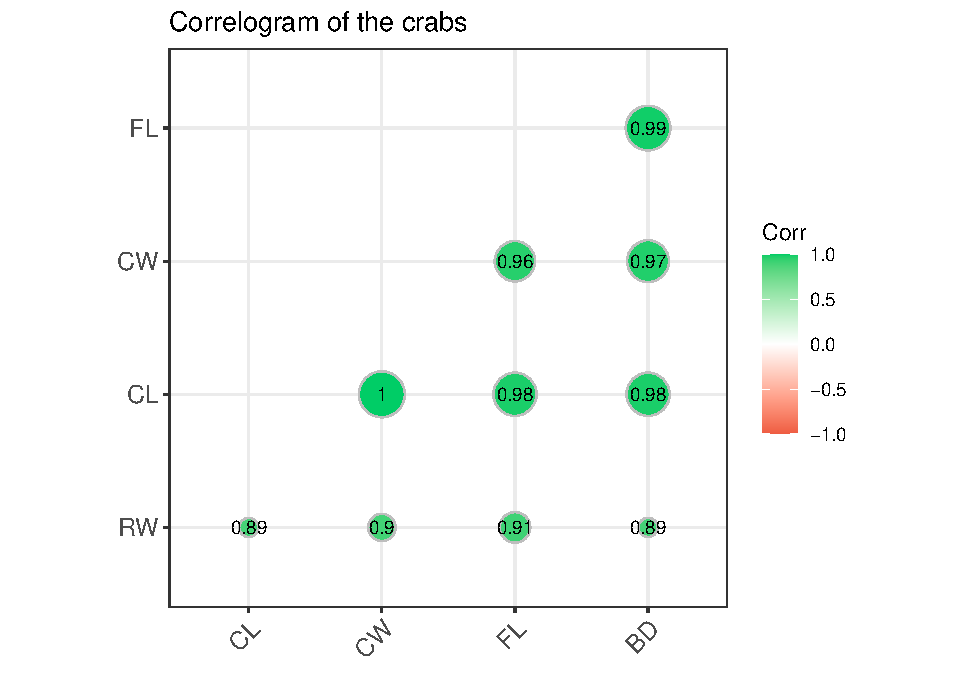
\includegraphics{CrabProject_files/figure-latex/unnamed-chunk-1-1} \end{center}

In the plot above the correlation between all the numerical elements of
the data set are shown, this has been done to be able to answer the
previously arisen question whether or not the data is correlated.

As seen in the plot above, the data inside the data set does indeed seem
to correlate which supports the earlier findings, this could mean that
there is more then one good attribute to be able to confidently support
the investigation of the research question

\begin{figure}[H]

{\centering 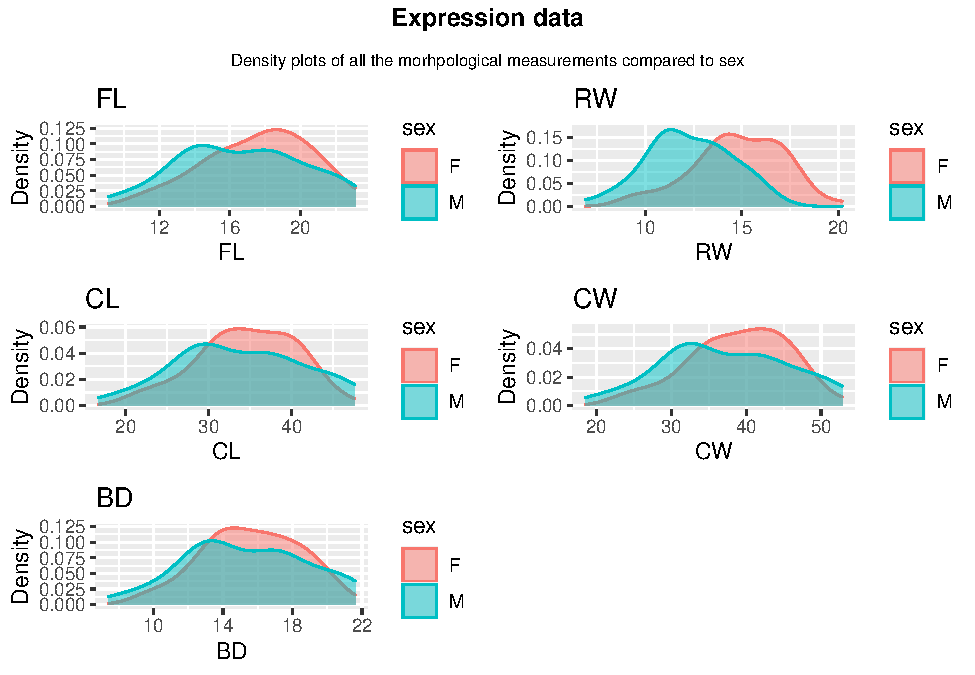
\includegraphics{CrabProject_files/figure-latex/figure6-1} 

}

\caption{Checking if the gender makes a difference}\label{fig:figure6}
\end{figure}

As seen in figure six, the orange crabs their morphological measurements
have been taken to be able to see if the sex matters when it comes to
the colours of the crabs,

\begin{center}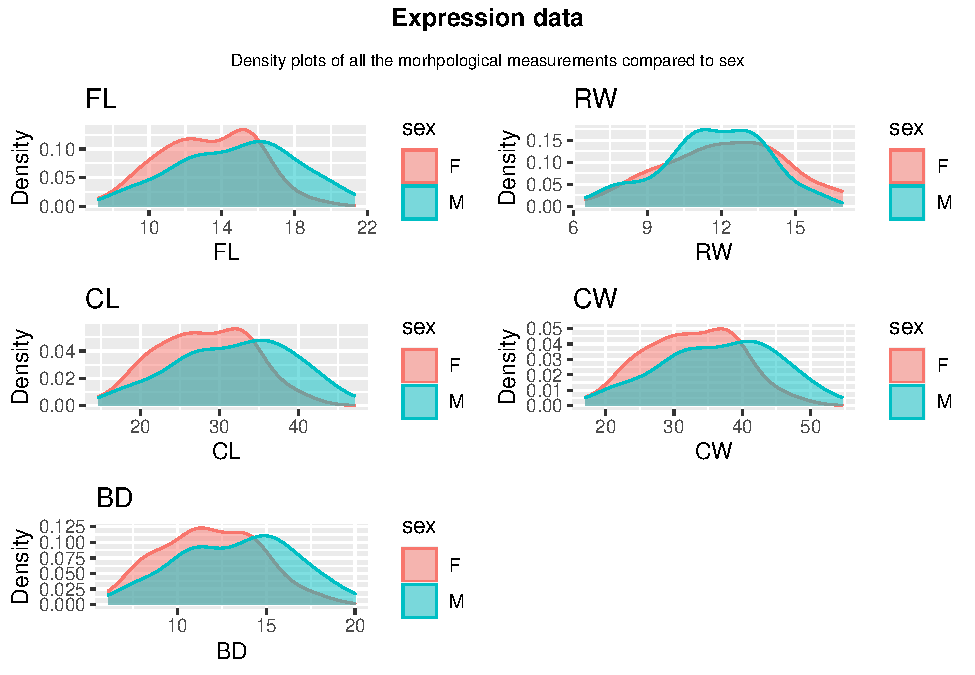
\includegraphics{CrabProject_files/figure-latex/figure 7-1} \end{center}

In figure six and seven the morphological variables of both color crabs
have been put into a density plot to see if there is any correlation
there, here it is however clearly visible these two separate colors
differ in their measurements. As can be seen in figure six: There are no
real differences with the morphological measurements for the orange
crabs, apart from the rear width, and here the females are noted to have
a larger rear width, apart from that some males appear to be on the
lager side of the spectrum in the density plot, but this does not seem
significant enough that it is to be mentioned. The orange crabs also
seem to have somewhat of a normal distribution or bell curve when it
comes to their measurements, this could indicate that they are either
smaller or their morphological components are more formed to each other.

In figure seven the blue crabs are depicted, here differing from figure
six, the male crabs of the blue species seem to be bigger in almost all
aspects of the morphological components apart from rear width, this
would indicate that for this species the male variant is bigger then the
female variant, how ever, this is a data set with only 100 crabs per
species and for a correct distribution a much larger sample size should
be taken. For the carapace length, it seems that for this species alone
it would be very good to be determined if the crab was of significant
size, which species it would belong to. To see if this would work with a
machine learning algorithm, further testing will need to be done.

\begin{center}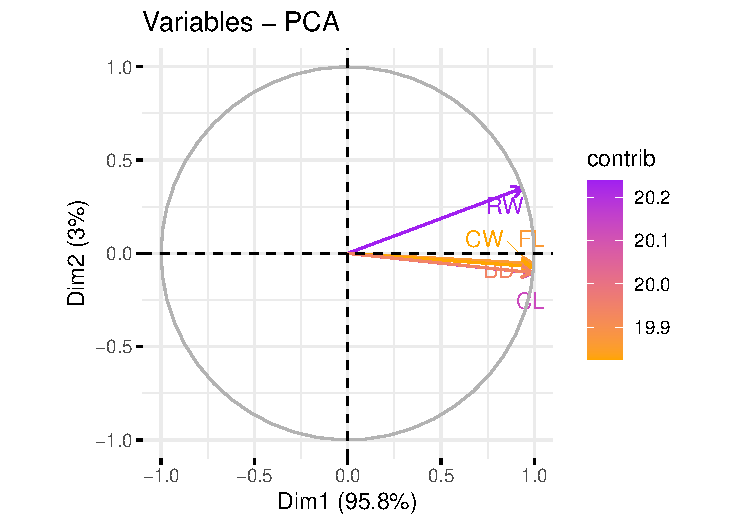
\includegraphics{CrabProject_files/figure-latex/pca-1} \end{center}

This PCA plot shows that the variables are highly correlated. The least
correlated variable is the Rear width. This vector has the largest angle
with the Carapace length, the same two variables were used to discover
the difference in carapace length distribution between the genders.

\hypertarget{machine-learning}{%
\subsubsection{Machine learning}\label{machine-learning}}

To find out what machine learning algorithm is the best for predicting
the species of crab, multiple algorithms were tested. These algorithms
are ZeroR, OneR, Simple logistic, Naive bayes, Random forest, J48, SMO
and K-nearest neighbor. These algorithms were tested using 10 fold
cross-validation. The highest quality metric for this data set is the
accuracy, since it does not matter whether a blue crab is predicted to
be orange, or an orange crab to be blue. The software used to calculate
the accuracy is WEKA. After the classification, the accuracy of these
algorithms was saved in a csv file, and are shown in this bar plot
below.

\begin{figure}[H]

{\centering 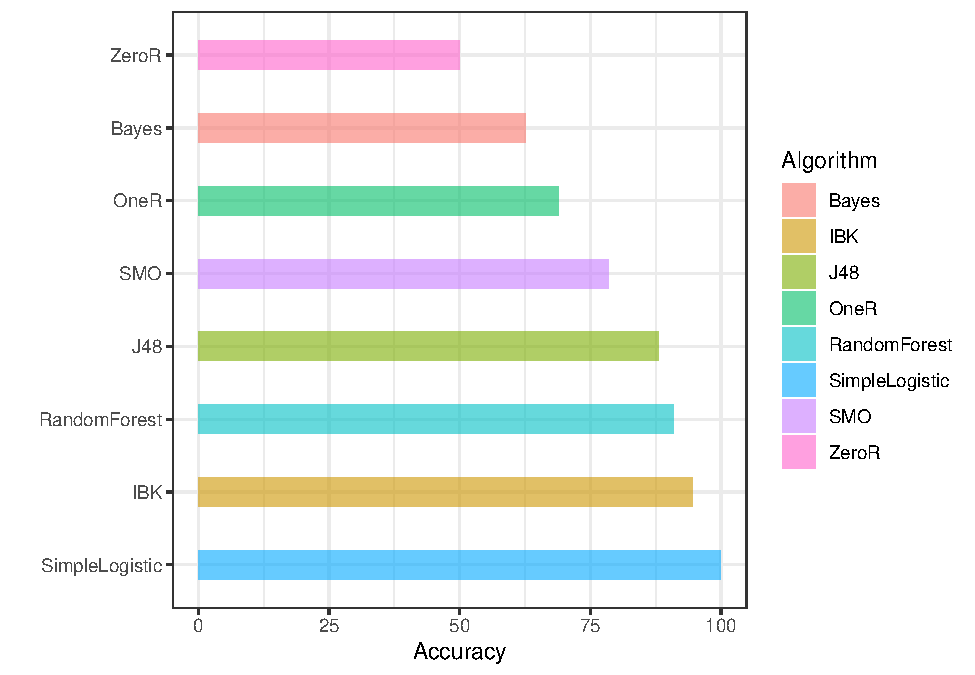
\includegraphics{CrabProject_files/figure-latex/ml-1} 

}

\caption{The accuracy of the machine learning algorithms ordered from low to high.}\label{fig:ml}
\end{figure}

This plot shows a few interesting things, most notably the 100\%
accuracy of Simple logistic. The output in weka of the classification
using Simple logistic with 10 fold cross-validation shows a model for
each species. The model for the blue crabs shows 1.03 + {[}FL{]} * -0.6
+ {[}CW{]} * 0.31 + {[}BD{]} * -0.22. The model for the orange crabs
shows -1.03 + {[}FL{]} * 0.6 + {[}CW{]} * -0.31 + {[}BD{]} * 0.22. The
values in the model of the orange crabs are the values of the model of
the blue crabs times -1. The metrics used in the models are Front lobe
size, Carapace width and Body depth. The barplot also shows an exact
50\% accuracy for the ZeroR algorithm. This is expected since the data
has the same amount of blue crabs as orange crabs.

\begin{center}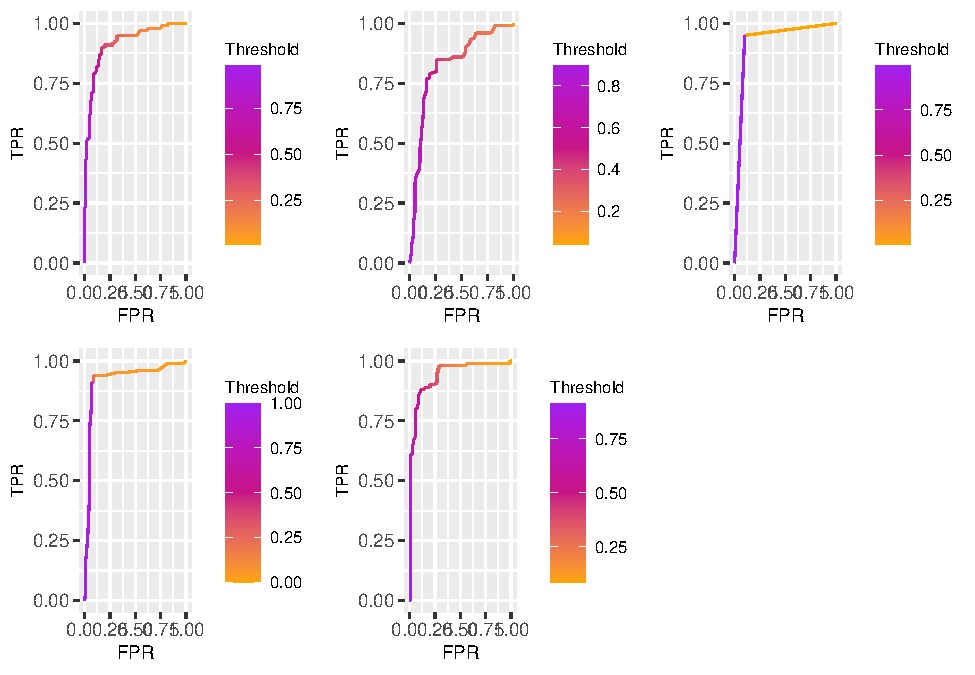
\includegraphics{CrabProject_files/figure-latex/unnamed-chunk-2-1} \end{center}
\newpage

\begin{center}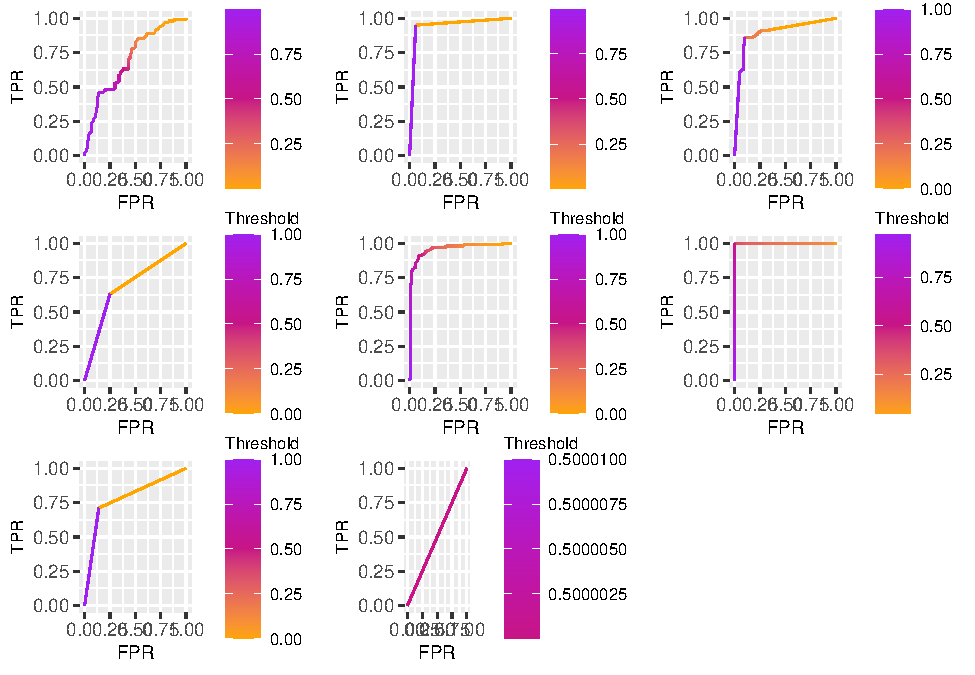
\includegraphics{CrabProject_files/figure-latex/rocs of algorithms-1} \end{center}

\begin{figure}[H]

{\centering 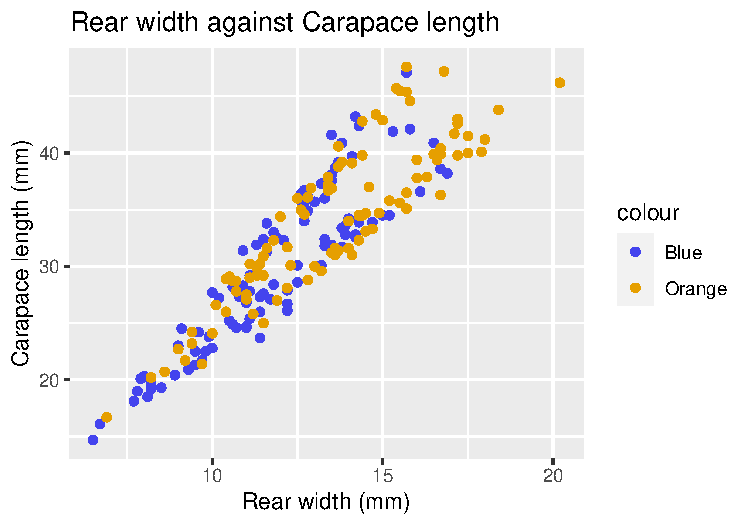
\includegraphics{CrabProject_files/figure-latex/unnamed-chunk-3-1} 

}

\caption{The metalearners: Stacking, Boosting, Bagging, Voting and Randomization}\label{fig:unnamed-chunk-3}
\end{figure}

\newpage

\hypertarget{conclusion-discussion}{%
\section{Conclusion \& Discussion}\label{conclusion-discussion}}

The goal was to get the dataset ready for machine learning. The data was
analyzed and cleaned to make so it is ready to be used in machine
learning algorithms. The data does not contain many outliers. The data
points seem easy to classify since most plots show clear groups of blue
and orange crabs. As shown in figure 4, the gender of the crab could
also be a good attribute to help predict the species of crab. The data
also had to be cleaned. This was done by removing the index column,
since this column can not be used to help determine the species of crab.
It might also be a problematic attribute for some machine learning
algorithms. Then, the species column was moved to the last column, so
the machine learning algorithms will use this column as the class index.

\hypertarget{future-work-proposal}{%
\section{Future work proposal}\label{future-work-proposal}}

Future research can be used to show more correlation between other
measurements. It can be researched whether or not the gender of the crab
could be predicted using these morphological measurements. Machine
learning use could also be improved by expanding the dataset, or getting
different amounts of blue or orange crabs, with different amounts of
male and female crabs.

\newpage

\hypertarget{sources}{%
\section{Sources}\label{sources}}

\hypertarget{references}{%
\subsection{References}\label{references}}

{[}1{]} Campbell, N.A. and Mahon, R.J. (1974) A multivariate study of
variation in two species of rock crab of genus Leptograpsus. Australian
Journal of Zoology 22, 417--425.

\hypertarget{github-repositories}{%
\subsection{Github repositories}\label{github-repositories}}

Link to the report and log repository:
\url{https://github.com/IJsbarnd/CrabWrapper}

Link to the java wrapper repository:
\url{https://github.com/IJsbarnd/thema9_2}

\end{document}
